\documentclass[conference]{util/IEEEtran}
\pagestyle{plain}

\let\proof\relax 
\let\endproof\relax
\usepackage{float}
\usepackage{amsmath,amsthm}

\usepackage[T1]{fontenc}
\usepackage[spanish, es-noshorthands]{babel}
\usepackage[utf8]{inputenc}
\usepackage{csquotes}
\usepackage[style=numeric,sorting=none,backend=biber]{biblatex}
\usepackage{tabularx}
\usepackage{pdflscape}
\usepackage{listings}
\usepackage{subfigure}
\usepackage{array}
\usepackage{perpage}
\usepackage{backnaur}
\usepackage{enumerate}
\usepackage{graphicx}
\usepackage{tikz}
\usepackage{tkz-kiviat}
\usepackage[bookmarks]{hyperref}
\usepackage{booktabs}
\usepackage{rotating}
\usepackage{glossaries}
\usetikzlibrary{shapes,arrows}


\MakePerPage{footnote}
\addbibresource{../bibliography.bib}

\newcommand{\foreign}[1]{{\it #1}}
\renewcommand{\thesubsection}{\Alph{subsection}}
\DeclareMathOperator*{\argmax}{arg\,max}
\renewcommand{\thetable}{\arabic{table}}


\makeatletter
\long\def\@makecaption#1#2{\ifx\@captype\@IEEEtablestring%
\footnotesize\begin{center}{\normalfont\footnotesize #1}\\
{\normalfont\footnotesize\scshape #2}\end{center}%
\@IEEEtablecaptionsepspace
\else
\@IEEEfigurecaptionsepspace
\setbox\@tempboxa\hbox{\normalfont\footnotesize {#1.}~~ #2}%
\ifdim \wd\@tempboxa >\hsize%
\setbox\@tempboxa\hbox{\normalfont\footnotesize {#1.}~~ }%
\parbox[t]{\hsize}{\normalfont\footnotesize \noindent\unhbox\@tempboxa#2}%
\else
\hbox to\hsize{\normalfont\footnotesize\hfil\box\@tempboxa\hfil}\fi\fi}
\makeatother


\newtoks\customtok


\renewcommand*{\newacronymhook}{%
 \edef\dosetkeys{\noexpand\setkeys{glossentry}{user1={},\the\glskeylisttok}}%
 \dosetkeys
 \ifcsempty{@glo@useri}%
 {%
   \expandafter\customtok\expandafter{\the\glsshorttok}%
 }%
 {%
   \edef\custom{\the\glsshorttok, \csexpandonce{@glo@useri}}%
   \expandafter\customtok\expandafter{\custom}%
 }%
}

\newcommand*{\custompostdesc}[1]{%
  \ifcsempty{glo@#1@useri}{}{(\glsentryuseri{#1})}%
}

\renewcommand*{\CustomAcronymFields}{%
  user1={},%
  name={\the\glsshorttok},%
  description={\the\glslongtok\noexpand\custompostdesc{\the\glslabeltok}},%
  first={\the\glslongtok\space(\the\customtok)},%
  firstplural={\the\glslongtok\noexpand\acrpluralsuffix\space(\the\customtok)}%
  text={\the\glsshorttok},%
  plural={\the\glsshorttok\noexpand\acrpluralsuffix}%
}

\makeglossaries

\begin{document}

\newacronym[user1=Conseil Européen pour la Recherche Nucléaire]{cern}{CERN}{Organización Europea para la Investigación Nuclear}
\newacronym[user1=One Laptop Per Child]{olpc}{OLPC}{Una computadora por niño}
\newacronym[user1=Massachusetts Institute of Technology]{mit}{MIT}{Instituto Tecnológico de Massachusetts}
\newacronym{tic}{TIC}{Tecnologías de la información y la comunicación}
\newacronym[user1=Event-Condition-Action]{eca}{ECA}{acciones condicionadas por eventos}
\newacronym{iab}{IAB}{Instituto Doctor Andrés Barbero}
\newacronym{fpuna}{FP-UNA}{Facultad Politécnica de la Universidad Nacional de
    Asunción}
\newacronym{una}{UNA}{Universidad Nacional de Asunción}
\newacronym[user1=Graphics Processing Unit]{gpu}{GPU}{Unidad de procesamiento de gráficos}
\newacronym[user1=Application Programming Interface]{api}{API}{Interfaz de programación de aplicaciones }
\newacronym[user1=Java Edici\'on Empresarial]{javaee}{JavaEE}{Java Enterprise Edition}
\newacronym[user1=Transferencia de Estado Representacional]{rest}{REST}{Representational State Transfer}
\newacronym[user1=Notación de objeto de JavaScript]{json}{JSON}{JavaScript Object Notation}
\newacronym[user1=Entorno de desarrollo Integrado]{ide}{IDE}{Integrated development environment}
\newacronym[user1=Licencia pública General GNU]{gnu}{GNU}{GNU General Public License}
\newacronym[user1=Licencia pública General de Affero GNU]{agnu}{AGNU}{GNU Affero General Public License}
\newacronym{gui}{GUI}{Interfaz gráfica de usuario}
\newacronym{udk}{UDK}{Unreal Development Kit}
\newacronym[user1=Lo que se ve es lo que se obtiene]{wysiwyg}{WYSIWYG}{What you
    see is what your get}
\newacronym{nombre}{eTesai}{eTesai}



\title{Juego serio como apoyo a la enseñanza tradicional:  una
	aplicación a la formación de profesionales del área de enfermería}

\author{\IEEEauthorblockN{Mirta González}
\IEEEauthorblockA{Facultad Politécnica\\
    Universidad Nacional de Asunción\\
    San Lorenzo, Paraguay\\
    Email: mirti.gonz@gmail.com}
\and
\IEEEauthorblockN{Arturo Volpe}
\IEEEauthorblockA{Facultad Politécnica\\
    Universidad Nacional de Asuncién\\
    San Lorenzo, Paraguay\\
    Email: arturovolpe@gmail.com}}

\maketitle
\thispagestyle{plain}


\begin{abstract}
%Lo fundamental de todo proceso pedagógico es el aprendizaje y no la enseñanza.
%Es el aprendizaje del estudiante y su participación el logro deseado.

Este trabajo introduce el uso de las TICs en forma de juegos serios como 
área de investigación. Se da una breve reseña de la inclusión de las 
tecnologías en la educación, desde su uso tradicional como proveedor de información hasta su rol actual en la construcción de conocimiento. 

Posteriormente se describen las principales características y áreas de 
aplicación de los juegos serios como herramienta educativa. Para luego 
introducirlo como solución tecnológica a las problemáticas del área de 
enfermería, las problemáticas y los detalles de la solución en forma 
de juego serio también son descritas.

Finalmente, se detallan las metodologías utilizadas para evaluar la 
solución junto con los resultados obtenidos más importantes. Estos resultados 
junto con la experiencia de desarrollar la solución permiten
obtener conclusiones e identificar posibles trabajos futuros en al área por lo 
que son detallados como parte final de este documento.



\end{abstract}

\begin{IEEEkeywords}
    Juego serio, simulación, enfermería, educación, ubicuidad, aprendizaje, 
    construccionismo, tecnologías de la información y la educación. 
\end{IEEEkeywords}


% La evaluación
% Un párrafo de Unity
% Resumir las escenas (General, objetivo, gráfico)
% Media página de TICS
% Media página de juegos serios
% Mencionar lo que se usa en la evaluación
% Población (Los tres gráficos)
% Abstract

% Objetivos
% Media página tics
% 1/2 página problema
% 1 Párrafo Unity
% 1 Página Arquitectura
% Ejemplos escenas (que se hace y objetivos)
% 1/2 evaluación
%%  Población (3 gráficos)
%%  Correlación
%%  Factores
% Conclusiones

\section{Introducción}
\setcounter{sectiontotal}{3}

\begin{frame}
\frametitle{\pagetitle}
\framesubtitle{Descripción}
\begin{figure}
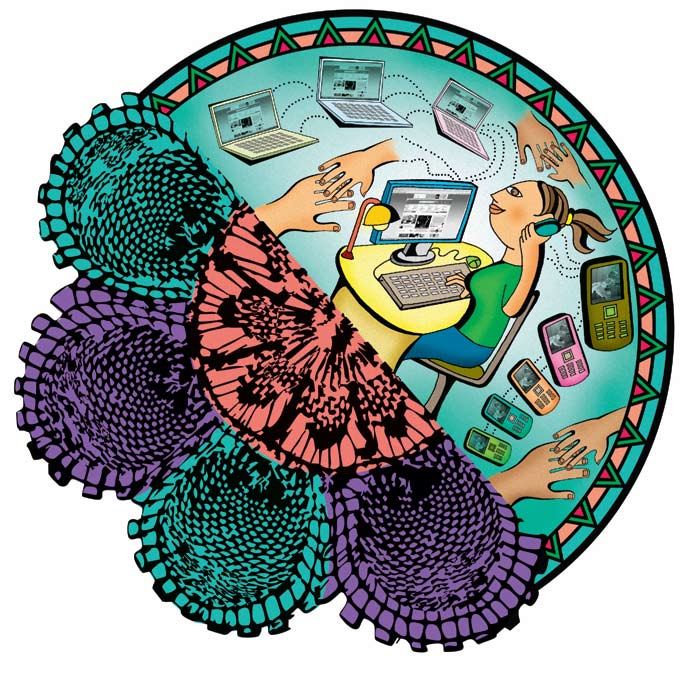
\includegraphics[scale=.3]{imagenes/nhanduti}
\end{figure}
\end{frame}

\begin{frame}
\frametitle{\pagetitle}
\framesubtitle{Objetivo general}
\begin{block}{Descripción}
\centering
Identificar y valorar los aspectos pedagógicos, de diseño, de implementación y
de evaluación que influyen a la creación de herramientas educativas que utilizan
las corrientes pedagógicas actuales apoyadas en las TIC, especialmente los
juegos serios.
\end{block}


\end{frame}

\begin{frame}
\frametitle{\pagetitle}
\framesubtitle{Objetivos específicos}

\small
\begin{itemize}[<+->]
\item Proveer una visión actualizada de las corrientes pedagógicas apoyadas con las TIC.
\item Proveer una visión actualizada de los juegos serios.
\item Identificar áreas de aplicación de los juegos serios.
\item Seleccionar las herramientas tecnológicas disponibles para el desarrollo de juegos serios.
\item Contrastar en la práctica los conocimientos teóricos adquiridos a través del diseño
e implementación de un juego serio.
\item Evaluar la solución propuesta para identificar los
aspectos de diseño, desarrollo y evaluación de los juegos serios.
\end{itemize}
\end{frame}


\section{\Gls{tic} en la educación}
%1/2 página

Las \Gls{tic} son un conjunto de herramientas tecnológicas y recursos utilizados para
comunicar, crear, diseminar, almacenar y manejar la
información\cite{unesco:ict}. Estas tecnologías abarcan computadoras
personales,internet, radio, televisión y telefonía\cite{tinio:ict} entre otros.

La utilización actual de las \Gls{tic} en la educación no es un fenómeno aislado,
responde a una evolución constante de la tecnología y metodología utilizada.
Existen cuatro pedagogías de entre varias en las que las tics han sido
utilizadas de manera activa, las cuales son el instruccionismo o educación
tradicional, el conductismo, el constructivismo y finalmente, el
construccionismo. Esto no implica que las tics no puedan ser aplicadas a otras
pedagogías, es más, existen otras corrientes que utilizan las \Gls{tic}, de diversas
maneras como el cognoscitivismo\cite{egenfeldt2007third} y el
conectivismo\cite{white:ict}. 

Este trabajo se basa en el construccionismo, pedagogía según la cual el
conocimiento es construido por el estudiante en lugar de ser trasmitido por el
profesor\cite{moses:2003} y esto sucede particularmente cuando el mismo se
involucre en la elaboración de un producto o artefacto que tenga un significado
y pueda ser compartido\cite{valdivia:sg}. El construccionismo y las tics siempre
han estado relacionados, ya que el mismo se originó con un lenguaje de
programación (LOGO)\cite{ict:ttc}. Posee un enfoque diferente en cuanto al uso
de las tics en la educación. Esta pedagogía se diferencia de la educación
tradicional en que el estudiante ya no es un receptor pasivo de información, en
cambio, el mismo participa activamente del proceso de aprendizaje construyendo
su propio conocimiento. Se diferencia del instruccionismo en que el
construccionismo utiliza la tecnología como medio cognitivo y no para la entrega
de contenido.

%\begin{itemize}
%\item Que son
%\item Educacion tradicional y mencionar las otras corrientes
%\item Construccionismo
%\end{itemize}
\section{Serious Game}
\label{sec:tics_JUEGO_SERIO}

Un \emph{Serious Game} es un vídeo juego elaborado con el propósito primario que
no es el de entretener\cite{sg:aoverview}, sino tienen una finalidad educativa
explícita y cuidadosamente pensada, utiliza la tecnología y los conceptos de la
industria de los vídeo juegos para encontrar solución a problemas reales. Es
decir, se utilizan para definir los juegos que poseen una pedagogía incluida,
algún tipo de evaluación ya sea interna o externa y lo que hay que aprender
(contenido) integrado\cite{damien:sg}.

Los \emph{Serious Game} proveen una oportunidad muy importante para ayudar en la
enseñanza y desarrollo de profesionales, por que ayudan a crear el tipo de
educación que los adultos prefieren, proveen mecanismos para que los estudiantes
cometan errores y experimenten con sus ideas, con su conocimiento y con la
teoría en un ambiente protegido sin riesgos para la vida o la identidad. 

Los beneficios que brindan los \emph{Serious Game} se acentúan en la medida en
la que los mismos proveen entornos más completos en donde realmente se puedan
poner en práctica la teoría, esto ayuda a una comprensión más profunda del área
de interés.

La principal diferencia entre los \emph{Serious Game} y otras aplicaciones de
\emph{E-Learing} es su enfoque en la creación de una experiencia de aprendizaje
significativo, relevante y atractivo. En un \emph{Serious Game} existen metas
claras de aprendizaje pero las mismas se encuentran en un contexto significativo
en donde se deben aplicar los conocimientos y hacer uso de herramientas que
están a disposición para obtener éxito en la resolución de los problemas
presentados. Estos problemas se equilibran a través de la retroalimentación y
otras estrategias para mantener el interés del estudiante
\cite{papertian:const}.
%. Todo esto hace que en los \emph{Serious Game} el principal objetivo sea ganar
%el juego no aprender, sin embargo sólo se puede hacer esto dominando el
%aprendizaje

\fixme{El campo de los \emph{Serious Game} rechaza la idea de que los profesionales de
    la educación pueden ser reemplazados fácilmente}{Obs: que es cada sección?,
    un enfoque? Una técnica? Un buzzword?}, para ellos la labor de estos
profesionales es imprescindible para la reflexión y orientación del aprendizaje.
Es cierto que se puede llegar a aprender sin el apoyo de un profesional de la
educación pero se corre el riesgo de perder el enfoque y la eficacia
\cite{elearning:seiousgames}. 

El \emph{serious Game} no se trata de una modelo de aprendizaje pasajero. Varios
autores como \emph{Johan Huizinga}, \emph{Jean Piaget}, \emph{Wittgenstin} y
\emph{Seymour Papert} han reconocido su importancia  como objeto de aprendizaje.
Los juegos deben ser elaborados teniendo en cuenta el nivel cognitivo del
estudiante, es decir, su etapa de aprendizaje y en que el aprendizaje difiere de
acuerdo a la etapa de vida en la que se encuentre un estudiante. Mediante la
práctica repetida de actividades relacionadas al área de interés se desarrollan
habilidades y destrezas\cite{education:games}. 

\observacion{Se podría hacer una comparación? (entre todos)}

Los siguientes son ejemplos de algunas áreas que utilizan Serious Game:

\begin{description}

\item[Militar] Los primeros juegos a menudo se basaban en lucha o combate.
	Durante más de 30 años los juegos han sido reconocidos como herramientas
	factibles en el entrenamiento de militares. En 1996 fue lanzado un juego
	llamado \emph{Marine Doom} en donde la tarea de los jugadores era el
	aprendizaje de formas de ataque, conservación de municiones, comunicarse
	con eficacia, dar órdenes al equipo de trabajo entre otros. De esta
	manera tuvo lugar una forma de entrenamiento más atractivo, sin el
	costo, dificultad, riesgos e inconvenientes que implicaría el mismo
	entrenamiento en un entorno real. Además se podían crear situaciones que
	en el mundo real serían muy difíciles de replicar y donde los errores
	pueden ser catastróficos además, permite la repetición hasta alcanzar la
	maestría\cite{education:games}.


\item[Salud] Este tipo de juegos son cada vez mayores, los juegos de salud se
	utilizan para la formación de profesionales basada en la simulación. En
	2008 el Centro de Simulación Hollier en Birmingham, Reino Unido, realizó
	una prueba que permitió a médicos jóvenes experimentar y entrenar para
	diversos escenarios médicos a través de maniquíes virtuales como
	pacientes, de este modo el aprendizaje se da por la experiencia. En su
	disertación, Roger D. Smith, realizó una comparación entre la enseñanza
	tradicional y la formación mediante realidad virtual y el uso de
	herramientas basadas en la tecnología de juegos en cuanto a la cirugía
	laparoscópica. Como conclusión afirmó que lo último era más barato,
	requería menos tiempo y que permitió menos errores médicos cuando los
	médicos se presentaban en una cirugía real debido a, entre otras cosas,
	la posibilidad de repetición de la experiencia sin riesgo
	alguno\cite{education:games}.



\item[Juegos corporativos] Este tipo de juegos se han utilizado para la
	selección de personal, la mejora de comunicación entre los directivos y
	su personal de confianza, y la formación de nuevos empleados. Un ejemplo
	de estos juegos es el INNOV8 de IBM que ayuda en el entrenamiento de los
	estudiantes acerca de la gestión de procesos de negocios. Los Serious
	Game pueden ser utilizados incluso para elaborar planes de
	negocios\cite{education:games}. 

\end{description}


\section{Planteamiento del problema}
\setcounter{sectiontotal}{8}

\begin{frame}{Estado actual del Instituto Andrés Barbero}

%\begin{figure}
%    \begin{subfigure}[b]{.6\linewidth}
%        \centering
%        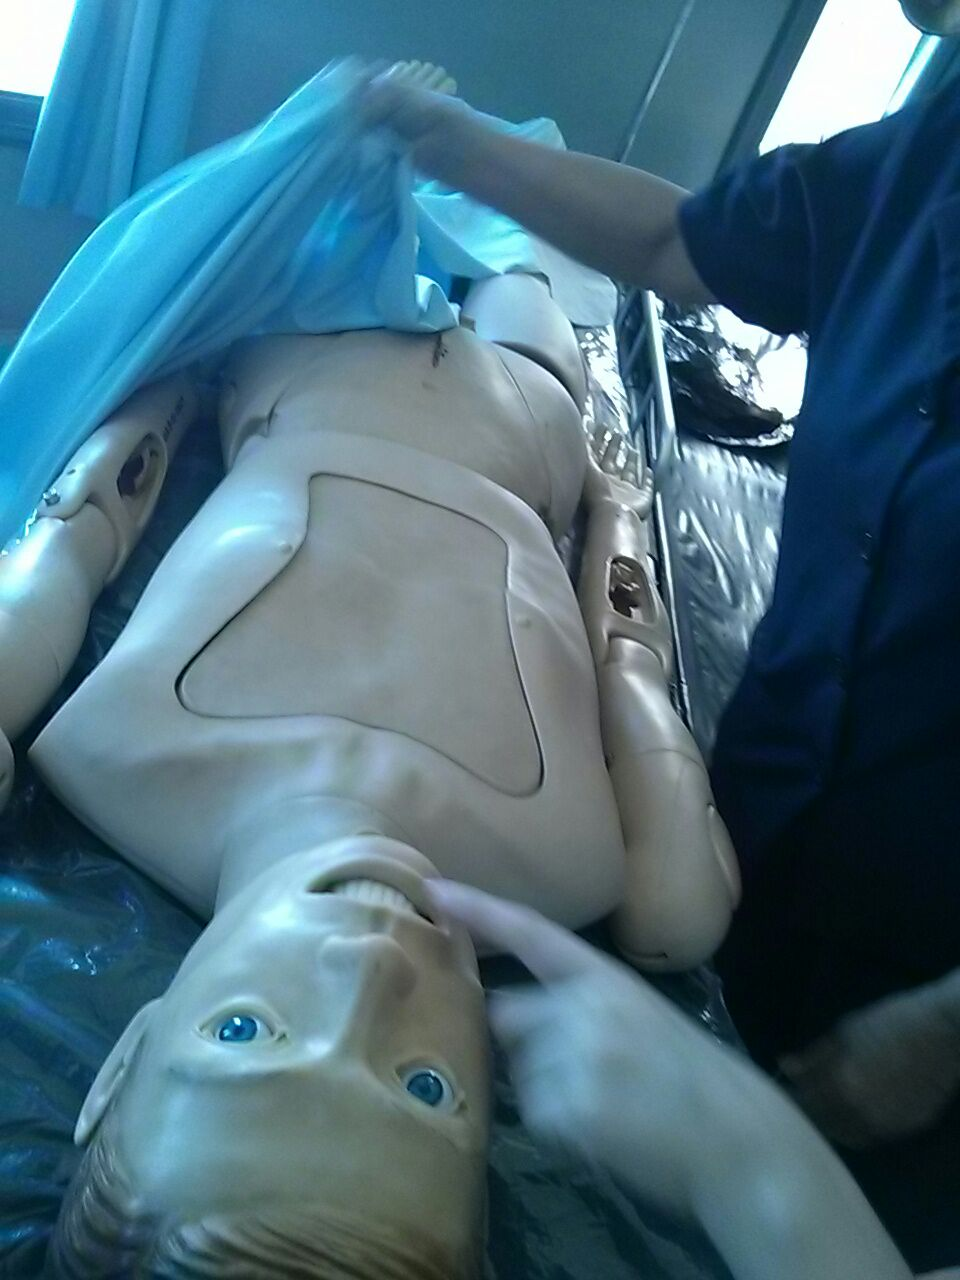
\includegraphics[height=3cm]{../problema/iab_sala_3.jpg}
%        \caption{Tiempo por tipo de actividad}
%    \end{subfigure}

    
%    \begin{subfigure}[b]{.6\linewidth}
	\begin{enumerate}[<+->]
	\item Prácticas en laboratorio
	\item Prácticas en hospitales o prácticas de campo
	\end{enumerate}
%	\end{subfigure}
%\end{figure}
\end{frame}

\begin{frame}{Problemas actuales del Instituto Andrés Barbero}
	\begin{enumerate}[<+->]
	\item Falta de preparación de los alumnos
	\item Definición de un protocolo de comunicación
	\item Nerviosismo ante la primera práctica
	\item Alta carga horaria de los trabajos prácticos
	\item Reducida carga horaria para el estudio de las materias teóricas
	\item Poca flexibilidad de los profesores
	\item Falta de materiales actualizados para los profesores
	\item Problemas de transporte
	\item Falta de preparación para las prácticas
	\item Alta cantidad de alumnos
	\end{enumerate}
\end{frame}

\begin{frame}{Propuesta de solución}
	\begin{enumerate}[<+->]
	\item Evaluación
	\item Progreso
	\item Tiempo de práctica
	\item Factor psicológico
	\item Ubicuidad
	\item Realismo
	\item Enfoque individual
	\end{enumerate}
\end{frame}

%\begin{frame}{Requerimientos de la solución}\end{frame}

\begin{frame}{Alcance de la solución (I)}
	Factores limitantes.
	\begin{enumerate}[<+->]
	\item Limitaciones técnicas
	\item Importancia de representación
	\item Facilidad de realización
	\end{enumerate}
\end{frame}

\begin{frame}{Alcance de la solución (II)}
	Hipótesis.
	\begin{enumerate}[<+->]
	\item Comando de voz con interfaz
	\item Extracción uniforme de elementos
	\item Acciones de bioseguridad
	\item Representación iconográfica
	\item Factores limitantes
	\item Falta de pistas
	\item Ubicuidad
	\end{enumerate}
\end{frame}

\begin{frame}{Alcance de la solución (III)}
	Decisiones de diseño.
	\begin{enumerate}[<+->]
	\item Acciones por interfaz de usuario
	\item Simulación integra de pasos
	\end{enumerate}
\end{frame}

%! TEX root = main.tex

\section{Solución}


Se diseña y desarrolla un Juego Serio para dispositivos móviles llamado
\textit{eTes\~{a}i}, el cual ofrece a los estudiantes de enfermería un medio para
realizar procedimientos de enfermería y cuyo objetivo es servir como herramienta
de apoyo al aprendizaje. La solución propuesta permite evaluar a los juegos
serios en los aspectos de diseño, implementación y evaluación.

%Los procedimientos simulados son seleccionados en conjunto con los profesionales
%del área de enfermería del \gls{iab} y son, la venopunción
%y la evaluación del paciente utilizando la escala de \textit{Glasgow}. 

\subsection{Arquitectura}

En la figura~\ref{fig:full_architecture} se observa la arquitectura general de la 
solución.

\begin{figure}[H]
\centering
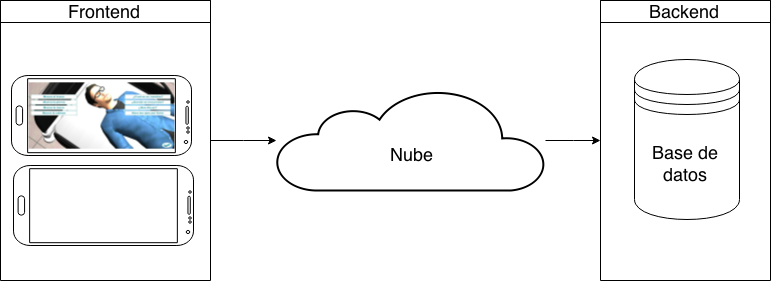
\includegraphics[scale=0.29]{images/full.png}
\caption{Esquema general de componentes de la solución.}
\label{fig:full_architecture}
\end{figure}

La solución se compone de un \textit{front-end}\footnote{El \textit{front-end}
    es la parte de la solución que interactúa con el usuario. Se encarga de
    realizar una simulación, de interpretar las acciones del usuario y evaluar
    el rendimiento del usuario.} que consiste en una aplicación \textit{Android}, la cual
es utilizada por los estudiantes de enfermería. Los registros de uso del
\textit{front-end} son almacenados bajo demanda en un servidor
\textit{back-end}\footnote{El \textit{back-end} es la parte de la solución que
    se encarga de almacenar la información de los usuarios y sus acciones dentro
    del \textit{front-end}.}, el cual se encarga de asociar los registros con
los alumnos y almacenarlos de manera persistente.

\subsection{Tecnologías utilizadas}

El motor de videojuegos utilizado para el desarrollo del \textit{front-end} es
\textit{Unity3D}, en su versión gratuita. \textit{Unity3D} es desarrollado por
\textit{Unity Technologies} y posee un motor de \textit{renderizado}, un flujo
de trabajo para la creación de contenido interactivo, y permite mezclar
contenido 3D, 2D, sonidos y animaciones en un entorno de desarrollo integrado.
\textit{Unity3D} permite desarrollar aplicaciones para múltiples sistemas
operativos, como \textit{Android, iOs, Windows Phone}, entre
otros\cite{unity3d}. El código fuente del \textit{front-end} es desarrollado con
\textit{MonoDevelop}.

% Agregar referencias
El \textit{back-end} es desarrollado utilizando \textit{Java EE 7}, servicios web
\textit{REST}, y \textit{Eclipse} como entorno de desarrollo integrado. 

\subsection{Front-end}

El \textit{front-end} consiste en una aplicación \textit{Android}, con un flujo que se observa en la
figura~\ref{fig:flujo_frontend}, la misma se inicia en la escena \emph{Inicio},
que permite al usuario seleccionar varias opciones y navegar a las demás
escenas.

\begin{figure}
\centering
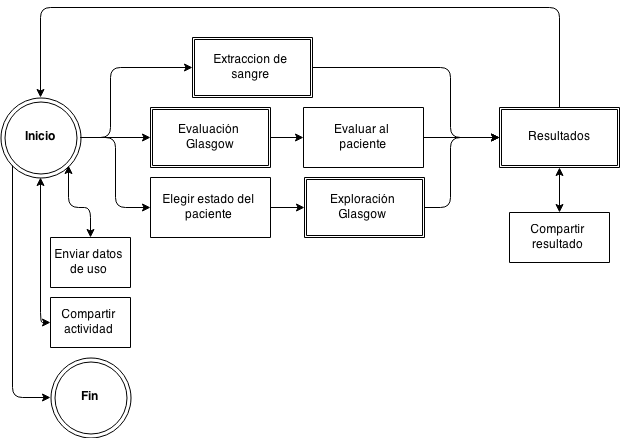
\includegraphics[width=8.5cm]{../solucion/images/grafo_escenas.png}
\caption{Flujo de pantallas de la solución}
\label{fig:flujo_frontend}
\end{figure}

La simulación posee dos mecanismos para interactuar con el punto de vista del
usuario, \textit{a)} alejar o acercar la cámara, y, \textit{b)} mover la cámara
alrededor del paciente.

Las acciones realizadas por los usuarios, así como el resultado de sus acciones,
son registradas en el dispositivo del usuario, y luego son enviadas al
\textit{back-end} para su persistencia.

\subsection{Back-end}

El servidor \textit{back-end} almacena la información del usuario, se encarga
de recibir y asociar los datos almacenados por el \textit{front-end} en una
base datos para su posterior análisis.


Almacena información detallada acerca de las acciones del usuario,
las condiciones de estas acciones y el contexto en el cual fueron ejecutadas.
La información almacenada permite reproducir las sesiones de juego
de los usuarios. Esta información es útil para analizar los puntos débiles y
fuertes, tanto de los usuarios como de la solución.

\subsection{Selección de procedimientos}

La selección de los procedimientos que forman parte de la solución se realiza
conjuntamente con los profesores del \Gls{iab} y son los siguientes:

\begin{itemize}
\item \textbf{Venopunción:} es utilizado frecuentemente para extraer muestras de
    sangre. Fue seleccionado debido a que: posee pasos bien definidos que deben
    ser seguidos por el profesional de enfermería, la complejidad del
    procedimiento no es muy alta y sus pasos son susceptibles de equivocaciones.
    El procedimiento formal, según los profesores del \gls{iab}
    y~\cite{oms:extraccion}, cuenta con $22$ pasos.
\item \textbf{Valoración de la escala de Glasgow:} es utilizada como una
    herramienta de valoración objetiva del estado de conciencia de pacientes en
    estado crítico. Consiste en la evaluación de la respuesta motora, verbal y
    ocular del paciente\cite{protocolo}. Fue seleccionado debido a que: permite
    la exploración del entorno pues hay diferentes formas de evaluar cada estado
    del paciente, rara vez es realizado pues las condiciones necesarias para que
    un paciente requiera que se le realice este procedimiento son críticas, la
    cantidad de reacciones que evalúa el procedimiento es muy alta y no es un
    procedimiento complejo. 
\end{itemize}

\subsection{Alcance}

Realizar una simulación de todos los aspectos que están presentes en un
procedimiento de enfermería es un proceso complejo. Cuando existe una gran
cantidad de detalles, los usuarios tienden a centrase en estos detalles y no en
los factores pedagógicos\cite{videojuegos:gonzaleztardon}, por esto, uno de los
objetivos de la solución es la presentación de situaciones simplificadas que
permitan construir conocimiento.

Las limitaciones técnicas\footnote{Las limitaciones técnicas se relacionan con
    la dificultad para simular un determinado paso, teniendo en cuenta
    consideraciones de \textit{hardware, software} y tiempo.}, la importancia de
la representación\footnote{La importancia de representación se refiere a que tan útil es
    un determinado paso para los objetivos pedagógicos.} y la facilidad de
realización\footnote{La facilidad de realización en la vida real
    se refiera a que tan fácil es realizar el paso en la vida real.} son los
factores utilizados para acotar el alcance de la simulación.

Algunas acciones requieren un esfuerzo significativo para ser simuladas y deben
formar parte del procedimiento. El nivel de detalle simulado para estas acciones
no es importante, por ello se formulan las siguientes consideraciones de diseño 
que permiten guiar la simulación de los mismos:


\begin{enumerate}[\bfseries C1.:]
%\begin{enumerate}[label=\bfseries H\arabic*:]

\item \textbf{Interacción a través de la voz}: para enviar una petición o
    informarle sobre algo al paciente, no es necesario utilizar reconocimiento
    del habla, sino más bien detectar que el usuario ha hablado y listar las posibles
    acciones que se puedan realizar. Los comandos de voz hacen más interactiva a
    la \gls{gui}.
    
\item \textbf{Extracción de elementos}: para realizar la acción de extraer un
    elemento utilizado en el paciente, se considera que realizarlo de una sola
    manera para todos los elementos disponibles en la solución aporta una
    interfaz más intuitiva.

\item \textbf{Bioseguridad}: la bioseguridad\footnote{La bioseguridad es la
        aplicación de conocimientos, técnicas y equipamientos para prevenir a
        personas, laboratorios, áreas hospitalarias y medio ambiente de
        exposición a agentes potencialmente infecciosos o considerados de riesgo
        biológico\cite{world2005manual}.} es un área amplia y transversal a
    todos los procedimientos de enfermería, por lo que se considera complejo
    simular cada acción. Es suficiente que el usuario sepa en que momento
    realizar cada una de las acciones. Realizar la simulación de todos los
    procedimientos de bioseguridad escapa al alcance del trabajo.

\item \textbf{Representación iconográfica}: para representar el estado de los
    objetos es suficiente mostrar una imagen representativa. Ciertos estados son
    complejos de simular (como la esterilización de las manos), realizar una
    simulación de los estados de los objetos es complejo y requiere un nivel de
    detalle que desviará al usuario de los objetivos pedagógicos.
    
\item \textbf{Motivación}: indicadores de rendimiento, como un puntaje al final
    de cada procedimiento, y el tiempo total dentro del procedimiento, impactan
    positivamente en el involucramiento del usuario. La interacción social es
    otro factor que incrementa el nivel de compromiso del usuario.

\item \textbf{Retroalimentación limitada}: la ausencia de signos visuales que
    indiquen las acciones que debe realizar el usuario durante la experiencia,
    permite al usuario probar sus conocimientos, y le impide avanzar en
    el procedimiento utilizando una técnica de \emph{prueba y error}.

\item \textbf{Movilidad}: el uso de la solución en los dispositivos móviles de
    los usuarios permite más oportunidades de poner a prueba los conocimientos
    con respecto a alternativas tradicionales.

\end{enumerate}

\subsection{Escenas}

La solución presenta procedimientos de enfermería en forma de escenas simuladas.
%Los procedimientos son seleccionados en conjunto con profesionales del área de
%enfermería del \gls{iab}. 

El procedimiento de venopunción, es representada dentro de la solución en la
escena \emph{Venopunción}. El procedimiento de evaluación de un paciente
utilizando la escala de \textit{Glasgow}, es representado en la escena
\emph{Glasgow}.

\subsection{Venopunción}

En la figura~\ref{fig:hemocultivo_principal} se observa el inicio de la escena,
el objetivo principal de este procedimiento es extraer muestras de la sangre del
paciente para su análisis en un laboratorio.

\begin{figure}[H]
\centering 
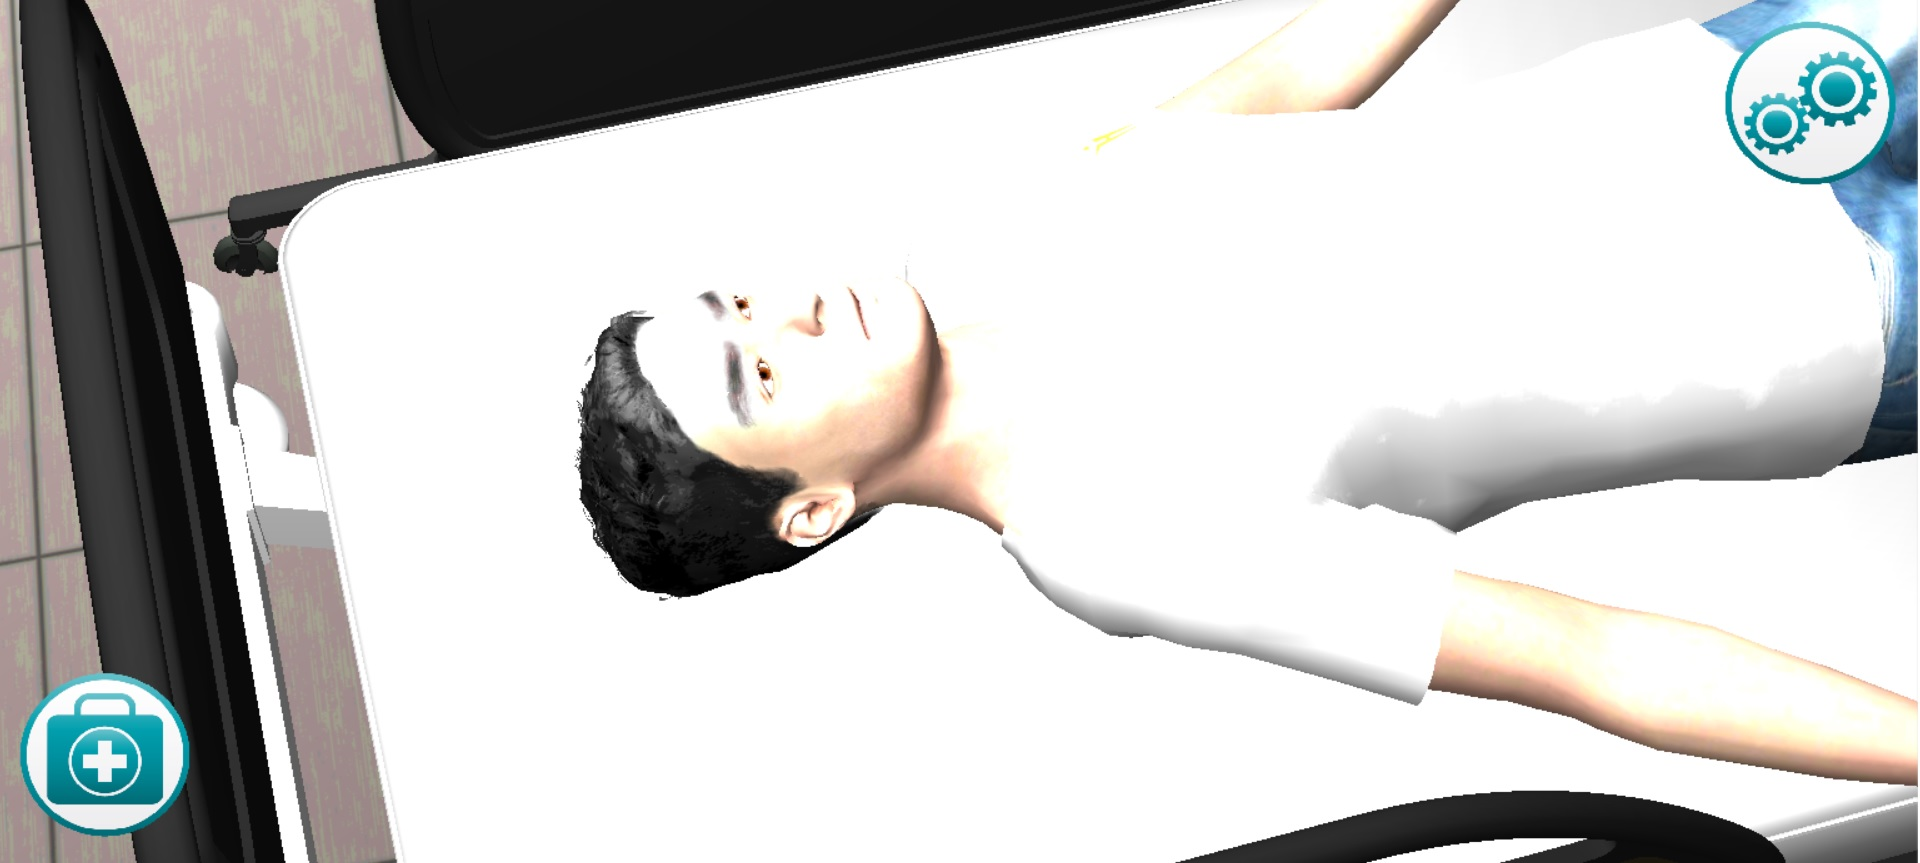
\includegraphics[width=8cm]{../solucion/images/hemocultivo_principal.jpg}
\caption{Pantalla principal de la escena \emph{Venopunción}.}
\label{fig:hemocultivo_principal}
\end{figure}

Durante la escena el usuario interactúa con varios objetos, en la
figura~\ref{fig:hemocultivo_jeringa_zoom} se observa la jeringa en el brazo del
paciente, con flechas ilustrativas que muestran como mover los dedos para
realizar la extracción de la sangre.

\begin{figure}[H]
\centering 
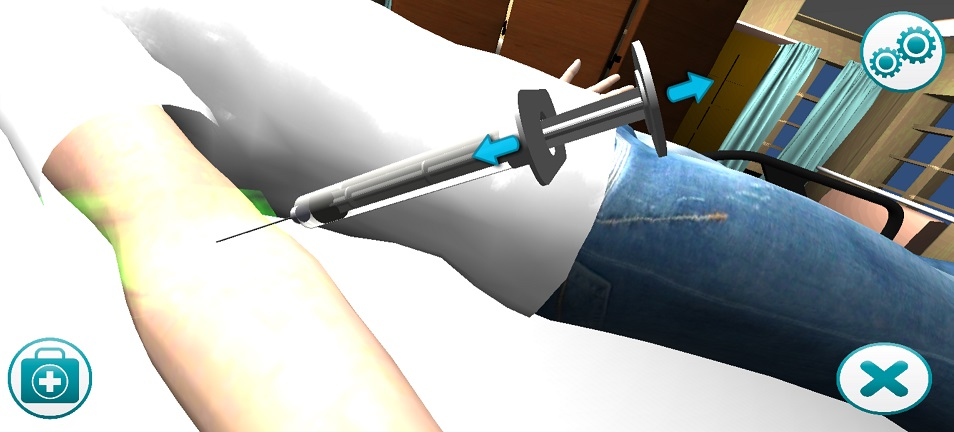
\includegraphics[width=8cm]{../solucion/images/hemocultivo_jeringa_ampliada.jpg}
\caption{Vista de la jeringa ampliada, facilitando la extracción de sangre.}
\label{fig:hemocultivo_jeringa_zoom}
\end{figure}

En la figura~\ref{fig:hemocultivo_gui} se observa la interfaz gráfica, con
opciones de bioseguridad y de utilización de elementos.

\begin{figure}
\centering
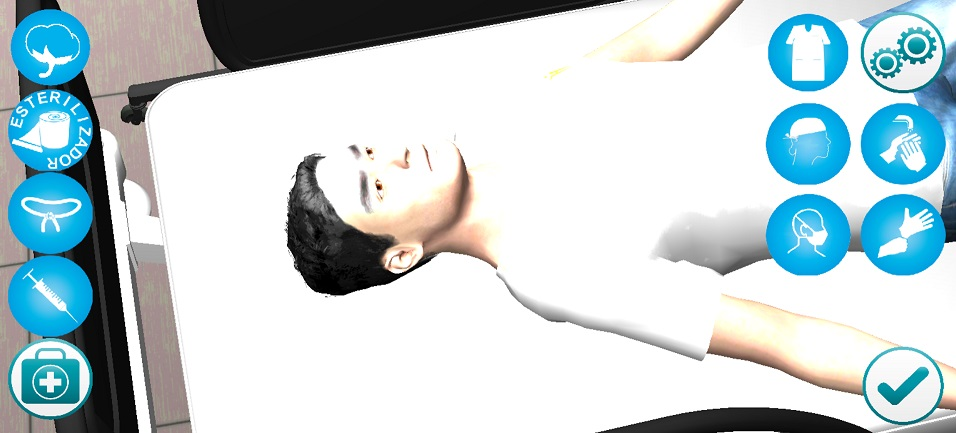
\includegraphics[width=8cm]{../solucion/images/hemocultivo_gui.jpg}
\caption{Interfaz gráfica de la escena \emph{Venopunción}}
\label{fig:hemocultivo_gui}
\end{figure}

La evaluación del desempeño del alumno durante la partida se utiliza un
motor de \gls{eca}\cite{bailey2004event,behrends2006combining}, este motor
permite reaccionar ante las acciones del usuario y verificar el cumplimiento de
los pasos del procedimiento. 

\begin{figure}
\centering 
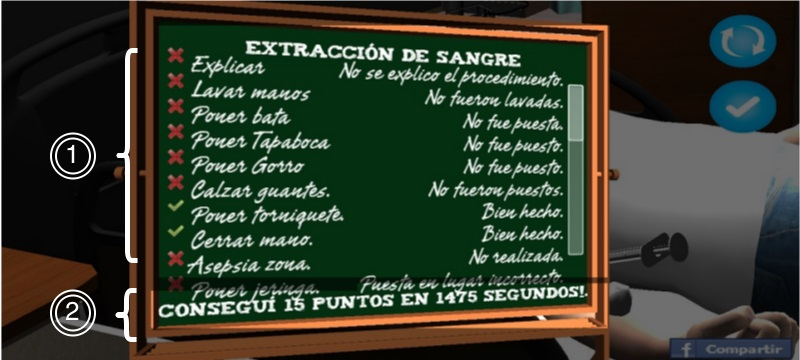
\includegraphics[width=8cm]{../solucion/images/hemocultivo_retroalimentacion.jpg}
\caption{Retroalimentación y puntuación final de la escena \emph{Venopunción}.}
\label{fig:hemocultivo_retroalimentacion}
\end{figure}

En la parte $1$ de la figura~\ref{fig:hemocultivo_retroalimentacion}, se observa
la información que la solución provee al usuario acerca de su rendimiento. Esta
información le indica los pasos que realizó de manera correcta o incorrecta y
las razones por las cuales tuvo ese desempeño.

Cada regla tiene asociado un peso, de acuerdo a la dificultad de realizar el
paso, este peso es utilizado al final de la partida para dar una puntuación al
usuario como se muestra en el punto $2$ de la
figura~\ref{fig:hemocultivo_retroalimentacion}. Junto al puntaje final también
se muestra el tiempo que le tomó al usuario completar el procedimiento.

\subsection{Glasgow}


%Permite al usuario explorar el entorno, es un procedimiento que requiere un
%%nivel alto de pericia, y solo algunos alumnos tienen la posibilidad de
%realizarlo durante las prácticas de campo debido a que requiere pacientes en
%estado crítico. 
El objetivo principal de esta escena es diagnosticar el estado de conciencia de
un paciente en estado crítico, utilizando la escala de \textit{Glasgow}. 

La interfaz principal se observa en la figura~\ref{fig:glasgow_principal}, se
observa al paciente a diagnosticar. Esta escena tiene dos versiones. La primera
versión, denominada \emph{Evaluación}, se inicia con un paciente en un estado
aleatorio, la tarea del alumno es diagnosticar el estado del paciente. En la
segunda versión, denominada \emph{Exploración}, el usuario elige el estado
inicial del paciente, lo que le permite observar como reacciona un paciente con
un diagnóstico dado.

\begin{figure}[H]
\centering
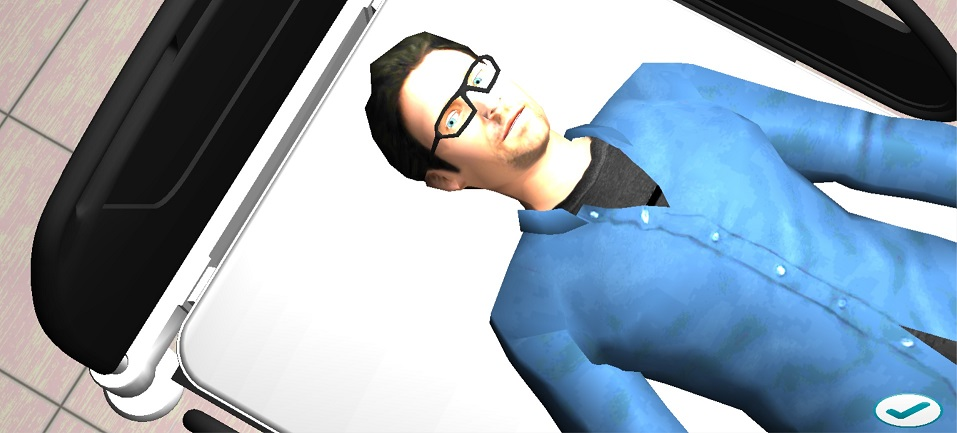
\includegraphics[width=8cm]{../solucion/images/glasgow_principal.jpg}
\caption{Interfaz de la escena de \emph{Valoración de la escala de Glasgow.}}
\label{fig:glasgow_principal}
\end{figure}



El protocolo indica que el enfermero debe valorar tres aspectos del paciente,
la visión (del $1$ al $4$), la audición (del $1$ al $5$) y la capacidad motora
(del $1$ al $6$)\cite{protocolo}. Realizada la valoración del
paciente, el enfermero debe sumar los puntajes obtenidos, y así realizar un
diagnóstico, de $13$ a $15$ el daño es leve, de $9$ a $12$ el daño es moderado y
de $3$ a $8$ el daño es severo\cite{helmick2007mild}.


\begin{figure}[H]
\centering
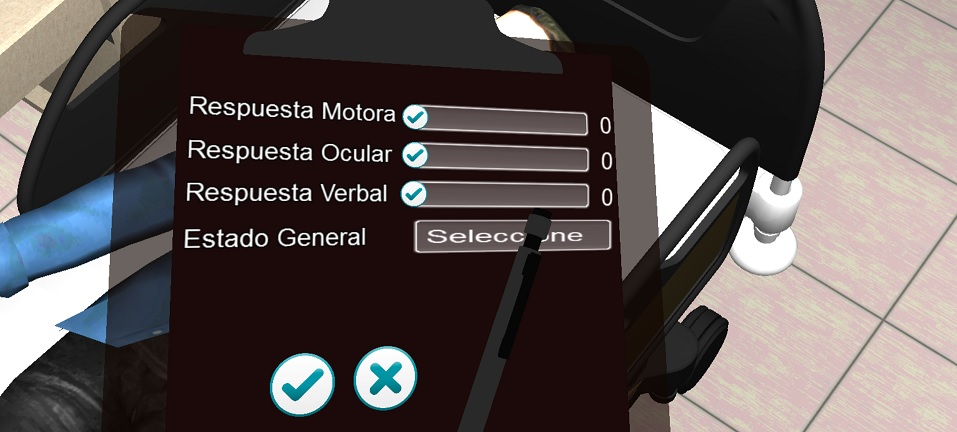
\includegraphics[width=7.5cm]{../solucion/images/glasgow_diagnostico.jpg}
\caption{Vista de la \emph{Pantalla de diagnóstico}.}
\label{fig:glasgow_gui_resultados}
\end{figure}

El diagnostico del usuario es contrastado con el estado real del paciente, para
mostrar el resultado de la escena, en el punto $1$ de la
figura~\ref{fig:glasgow_resultado} se observa la retroalimentación dada al
usuario.

Para el cálculo del puntaje final, por cada respuesta dada en la \emph{Pantalla
    de diagnóstico} se asigna una puntuación de acuerdo a que tan cerca estuvo
el usuario de la respuesta correcta. Se suman estos valores y se calcula el
porcentaje de acierto. El puntaje final junto al tiempo que tardó el usuario
realizando el procedimiento son presentados como se observa en el punto $2$ de
la figura~\ref{fig:glasgow_resultado}.

\begin{figure}[H]
\centering
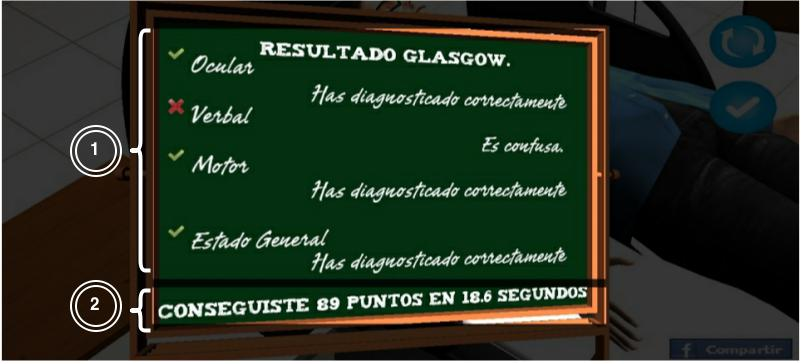
\includegraphics[width=7.5cm]{../solucion/images/glasgow_resultado.jpg}
\caption{Retroalimentación y puntuación final de la escena \emph{Glasgow}.}
\label{fig:glasgow_resultado}
\end{figure}

\section{Evaluación y resultados}

%En esta sección se explicarán las metodologías utilizadas para 
%evaluar la solución y los principales resultados obtenidos.
\begin{table}[H]
\centering
\caption{Metodologías utilizadas en la evaluación de la solución}
\begin{tabulary}{.5\textwidth}{RLLL}
\toprule
\textbf{Prueba}        & \textbf{Determinar la muestra} & \textbf{Evaluar el uso y la aceptación} & \textbf{Evaluar el conocimiento} \\
\midrule
\textbf{Participantes} & \multicolumn{3}{c}{Alumnos de la carrera de enfermería del IAB} \\
\midrule
\textbf{Muestra}       & 124 Alumnos                                                        & 11 Alumnos                     & 124 alumnos \\
\midrule
\textbf{Lugar}         & IAB                                                                &                                & IAB\\
\midrule
\textbf{Duración}      & 10 minutos                                                         & 20 días                        & 20 minutos\\
\midrule
\textbf{Fases}   & \tabitem Presentación. & \tabitem Explicación de la interfaz. & \tabitem Explicación de la prueba.\\
                 & \tabitem Encuesta.     & \tabitem Utilización de la solución. & \tabitem Encuesta sobre conocimiento\\
                 &                       & \tabitem Encuesta de apreciación.    & \\
\bottomrule
\end{tabulary}
\label{tab:metodologia}
\end{table}

En el cuadro~\ref{tab:metodologia} se observan las metodologías utilizadas
para la evaluación de la solución incluyendo la determinación de la muestra.

A continuación se describen los detalles de la metodologías utilizadas junto con
los principales resultados obtenidos.

%Comentarios de tincho:
% A quien se le hizo el test (muestra)
% Correlación
% Resumen de todo
% Encuesta objetiva
% Explicar a quien se le hizo el test, resumen, correlación
%3 paginas

\subsection{Encuesta para determinar la muestra}
\label{encuesta_muestra}

Con esta encuesta se determinó el nivel de acceso a la tecnología de los
estudiantes del cuarto año de Licenciatura en Enfermería del \gls{iab}, además
del tipo de acceso a Internet, sistema operativo de sus teléfonos móviles y si
cumplían con los requisitos técnicos para utilizar la solución. Estos requisitos
son los siguientes:  memoria RAM de $512MB.$ o superior, velocidad de procesador
de $800 GHz.$ o superior y tarjeta de video compatible con \emph{OpenGL ES 2.0}. 

\begin{figure}[H]
\centering
\begin{tikzpicture}[thick,scale=0.7, every node/.style={transform shape}]
    \pie[
        text=legend,
        explode=.1,
        style=drop shadow,
        ]%
    {%
        81.7 / No cumple,
        18.3 /  Cumple
    }
\end{tikzpicture}
\caption{Dispositivos que cumplen con los requisitos mínimos para la prueba}
\label{fig:ubicacion_requisitos_minimos}
% TODO se debe ver los requisitos en esta misma página.
\end{figure}

\begin{figure}[H]
\centering
\begin{tikzpicture}[thick,scale=0.7, every node/.style={transform shape}]
    \pie[
        %explode=.2,
        text=legend,
        style=drop shadow,
        %radius=3,
        %scale font,
        explode={0.1,0.1,0.3,0.3}
        ]%
    {%
        31.2 / Plan pos-pago,
        57   / Paquetes pre-pago,
        5.4  / Sin acceso,
        6.4  / Acceso ocasional}
\end{tikzpicture}
\caption{Acceso a internet desde dispositivos móviles}
\label{fig:ubicacion_acceso_internet}
\end{figure}

\begin{figure}[H]
\centering
\begin{tikzpicture}[thick,scale=0.7, every node/.style={transform shape}]
    \pie[
        text=legend,
        rotate=61.3,
        explode={.1,.2,.2,.2},
        style=drop shadow,
        ]%
    {%
    61.3 / Android,
     8.6 / Symbian,
    12.9 / Windows Phone,
    17.2 / Otros}
\end{tikzpicture}
\caption{Sistemas operativos móviles utilizados}
\label{fig:ubicacion_sistemas_operativos}
\end{figure}

Del $18.3\%$ de los que cumplían con los requisitos, $11$ alumnos estuvieron
dispuestos a evaluar la solución. 

El estudio~\cite{nielsen2000} establece que la cantidad de usuarios requeridos
para las pruebas de \gls{gui} dependen del nivel de experiencia de los usuarios
con tecnología similar, y~\cite{ritch2009} define el rango de usuarios
necesarios para resultados estadísticamente válidos, cuando los mismos no tienen experiencia con la tecnología, de $10$ a $12$.
% La muestra utilizada en las pruebas de la solución es de $11$ usuarios.

%\FloatBarrier

\subsection{Encuesta para evaluar la solución}
\label{encuesta_solucion}

Con esta encuesta se busca identificar las fortalezas y debilidades de la
solución, además de evaluar la solución en cuanto a factores de exploración,
representación, motivación, inmersión, retroalimentación y pedagogía. También se
busca valorar el nivel de aceptación de la solución y la validación de las
consideraciones de diseño planteadas como parte del diseño de la solución.

La encuesta cuenta con $27$ preguntas cerradas, es decir de una sola respuesta
en una lista de opciones, y con $4$ preguntas abiertas, es decir los encuestados
pueden dar respuestas libres a las preguntas. 

En las preguntas cerradas la métrica utilizada es la escala de Likert
\cite{Allen:2007} de 7 valores posibles cuyo valor más alto es
\enquote{Totalmente de acuerdo} y el más bajo es \enquote{Totalmente en
    desacuerdo}. 

Una vez valoradas y registradas todas las respuestas y con el 
objetivo de eliminar las tendencias en la forma en la que son completadas las
encuestas\cite{Fischer2010} se utiliza el método de \emph{Doble 
Estandarización} recomendado en~\cite{Pagolu2011}, el promedio estandarizado 
refleja los puntos fuertes y débiles relativos a la valoración más alta y baja.

En el cuadro~\ref{tab:resultado_resumen_aspectos_aceptacion} se observa 
la aceptación de los usuarios por aspecto estudiando. En el 
cuadro~\ref{tab:resultado_resumen_hipotesis} se observa la aceptación
de los usuarios por hipótesis asumida.  

\begin{table}[b]
\centering
\caption{Aceptación por aspecto de la solución}
\begin{tabulary}{.50\textwidth}{LRLL}
\toprule
\textbf{Factor}                   & \shortstack{\textbf{Promedio encuesta} \\ (Promedio estandarizado)} & \textbf{Puntos fuertes}             & \textbf{Puntos débiles} \\
\midrule
Motivación           & De acuerdo (0.67)              & \tabitem Puntaje                    & \tabitem Tiempo  \\
                     &                                & \tabitem Socialización              & \\
\midrule
Exploración          & De acuerdo (0.68)              & \tabitem Aleatoriedad               & \tabitem Utilización    \\
                     &                                & \tabitem Funciones                  & \\
\midrule
Inmersión            & De acuerdo (0.63)              & \tabitem Escenografía               & \tabitem Pertenencia\\
                     &                                & \tabitem Gráficos                   & \\
                     &                                & \tabitem Ordenes verbales           & \\
\midrule
Pedagogía            & De acuerdo (0.67)              & \tabitem Comprensión                & \\
                     &                                & \tabitem Retroalimentación limitada & \\
\midrule
Representación       & Parcialmente de acuerdo (0.53) & \tabitem Movimientos motrices       & \tabitem Reacción verbal\\
                     &                                &                                     & \tabitem Estados del paciente\\
\midrule
Retroalimentación    & Parcialmente de acuerdo (0.60) & \tabitem Detalles de los pasos      & \tabitem Iconos \\
                     &                                &                                     & \\
\midrule
Utilidad             & De acuerdo (0.69)              & \tabitem Complemento                & \tabitem Interacción \\
                     &                                & \tabitem Facilitador                & \\
\bottomrule
\end{tabulary}
\label{tab:resultado_resumen_aspectos_aceptacion}
\end{table}



\begin{table}
\centering
\caption{Consideraciones de diseño con su aceptación}
\begin{tabular}{lcr}
\toprule
Consideración de diseño     & Promedio encuesta     & Promedio estandarizado \\
\midrule
C1. Interacción a través de la voz  & De acuerdo              & $0,55$ \\
C2. Extracción de elementos & Parcialmente de acuerdo & $0,65$ \\
C3. Bioseguridad            & De acuerdo              & $0,58$ \\
C4. Representación iconográfica  & Parcialmente de acuerdo & $0,53$ \\
C5. Motivación              & De acuerdo              & $0,65$ \\
C6. Retroalimentación limitada      & De acuerdo              & $0,61$ \\
C7. Movilidad               & De acuerdo              & $0,66$ \\
\bottomrule
\end{tabular}
\label{tab:resultado_resumen_hipotesis}
\end{table}

%\begin{figure}
%\centering
%\begin{tikzpicture}[label distance=.15cm]
%\tkzKiviatDiagram[scale=.5,%
                    %lattice=9,
                    %%step=10,
                    %]
                %{Motivación,
                 %Exploración,
                 %Inmersión,
                 %Pedagogía,
                 %Representación,
                 %Retroalimentación,
                 %Utilidad}
%\tkzKiviatLine[thick,
                %color=blue!25!white,
                %mark=ball,
                %ball color=blue,
                %mark size=5pt,
                %opacity=.2, 
                %fill=blue!20](6.7,6.8,6.3,6.7,5.3,6.0,6.9)
%\tkzKiviatGrad[prefix={$0,$}](1) 
%\end{tikzpicture}
%\label{fig:subjetiva_kiviat}
%\caption{Gráfico de Kiviat de los factores evaluados}
%\end{figure}

\subsection{Encuesta para evaluar el conocimiento}

Esta encuesta mide el nivel de conocimiento de los alumnos sobre los dos temas 
simulados, contiene preguntas de nivel básico, medio y avanzado. Las mismas 
son formuladas utilizando la lista de competencias básicas que debe tener un 
alumno para aprobar la materia \textbf{Enfermería en Urgencias II}. Las 
preguntas son validadas  por los profesores de la cátedra. Cada pregunta 
tiene el mismo peso, así la puntuación más baja obtenible es $0$, y la más 
alta es $10$. La encuesta fue aplicada a la muestra y a un grupo de control 
compuesto por los demás estudiantes de la población objetivo.

De esta manera se busca evaluar la influencia pedagógica  de la solución en el
aprendizaje. Dado que la cantidad de partidas jugadas por usuario por tipo de
procedimiento no es considerada suficiente no se pueden considerar las
diferencias entre la muestra y el grupo de control como absolutas. En el
cuadro~\ref{tab:objetiva_rendimiento_por_pregunta} se observan los resultados de
esta prueba. %ver si agregar lo del metodo de evaluacion

\begin{table}[H]
\centering
\caption{Rendimiento promedio de usuarios por pregunta}
\begin{tabular}{lrrr}
\toprule
& \multicolumn{3}{c}{Promedio} \\
\cmidrule(lr){2-4}
\textbf{Pregunta} & 
\textbf{Muestra} & 
\textbf{Grupo Control} & 
\textbf{Total} \\ 
\midrule
ES1. Torniquete           & 0.36 & 0.18 & 0.20 \\
ES2. Guantes              & 0.64 & 0.60 & 0.60 \\
ES3. Manos                & 0.09 & 0.14 & 0.13 \\
ES4. Bioseguridad         & 0.27 & 0.25 & 0.26 \\
ES5. Explicación          & 0.82 & 0.56 & 0.59 \\
\midrule
EG1. Diagnóstico Global 1 & 0.00 & 0.18 & 0.16 \\
EG2. Diagnóstico Global 2 & 0.64 & 0.51 & 0.53 \\
EG3. Respuesta ocular     & 0.45 & 0.28 & 0.29 \\
EG4. Respuesta motora     & 0.18 & 0.32 & 0.31 \\
EG5. Respuesta verbal     & 0.36 & 0.45 & 0.45 \\
\midrule
\textbf{Sumatoria}: & 3.82 & 3.47 & 3.49  \\
\bottomrule
\end{tabular}

\label{tab:objetiva_rendimiento_por_pregunta}
\end{table}

\subsection{Registro de actividades}

La solución propuesta almacena información relacionada a la actividad del
usuario, incluyendo cuando y como utiliza las acciones, los pasos que realiza,
el orden y las condiciones de la escena cuando realiza cada acción, el tiempo de
partida por procedimiento, entre otras informaciones.

El registro de actividades ayuda a identificar las  fortalezas y debilidades de
la solución en cuanto al diseño y utilidad. Sobre todo, ayuda a medir el impacto
pedagógico al permitir contrarrestar el uso y desempeño del usuario con el
puntaje obtenido por el mismo en la encuesta utilizada para medir el
conocimiento. Los principales resultados obtenidos utilizando la correlación de
Pearson\cite{BoslaughStatistics2008} entre los datos del registro de actividades
y de la encuesta de conocimiento considerando sólo a la muestra son los
mostrados en el cuadro~\ref{tab:all_correlation}.

\begin{table}[H]
\centering
\caption{Correlación entre factores estudiados} 
\begin{tabular}{lrrrrrr}
\toprule
        &
\begin{sideways}\textbf{Puntaje Máx Venopunción (juego)}\end{sideways}  &
\begin{sideways}\textbf{Puntaje Máx Glasgow (juego)}\end{sideways}        &
\begin{sideways}\textbf{Tiempo Jugado Venopunción}\end{sideways}         &
\begin{sideways}\textbf{Tiempo Jugado Glasgow}\end{sideways} &
\begin{sideways}\textbf{Puntaje Venopunción (examen)}\end{sideways}  &
\begin{sideways}\textbf{Puntaje Glasgow (examen)}\end{sideways}    \\
\midrule
Puntaje Máx Venopunción (juego)    & 1    & 0.12  & \textbf{0.30}   & \textbf{0.35} & \textbf{0.74} & 0.55 \\
Puntaje Máx Glasgow (juego)       & 0.12 & 1     & 0.32 & \textbf{0.61} & 0 & \textbf{0.54}\\
Tiempo Jugado Venopunción     		 & \textbf{0.30}  & \textbf{0.32} & 1  & 0.29 & 0.04 & 0.05\\
Tiempo Jugado Glasgow 				 & \textbf{0.35} & \textbf{0.61}  & 0.29  & 1    & 0.69 & \textbf{0.86}\\
Puntaje Venopunción (examen) & \textbf{0.74} & 0 	& 0.04  & 0.69 & 1 & \textbf{0.78} \\
Puntaje Glasgow (examen)    		 & 0.55 & \textbf{0.54} & 0.05  & \textbf{0.86} & \textbf{0.78} & 1 \\
\bottomrule               
\end{tabular}

\label{tab:all_correlation}
\end{table}

%Las correlaciones fuertes, que se observan en el 
%cuadro~\ref{tab:all_correlation}, son:

%\begin{itemize}
%    \item Tiempo de uso y puntaje máximo extracción, $0,62$, correlación
%        positiva fuerte.
%    \item Tiempo de uso y puntaje máximo Glasgow, $0,78$, correlación positiva
%        muy fuerte.
%    \item Puntaje máximo extracción y encuesta conocimiento, $0,44$, correlación
%        positiva fuerte.
%\end{itemize}

%Estas correlaciones sugieren una relación entre el tiempo de uso de la solución
%y el puntaje obtenido en cada uno de los procedimientos, lo que sugiere que
%mientras más tiempo se dedico a la solución, mejor puntaje se obtuvo, indicando
%que los usuarios aprendieron a utilizarla.


% TODO FALTA ESTO


%Los tres gráficos (estos gráficos son de la ubicación)
%\subsection{Variables}
%\subsection{Resultados}
%\begin{itemize}
%\item Aceptación de la solución (estrella de kiviat)
%\item Correlación
%\end{itemize}

\section{Conclusiones}
\setcounter{sectiontotal}{7}

% Estado del arte
\begin{frame}
\frametitle{\pagetitle}
\framesubtitle{Estado del arte}
\begin{itemize}[<+->]

% REVISAR
\item Beneficios no explotados de las TIC

%\item El construccionismo y el constructivismo son pedagogías útiles para el
%desarrollo de habilidades profesionales

\item Los juegos serios permiten una experiencia sin riesgos

%\item Los juegos serios actuales ofrecen una retroalimentación muy guiada

\item La enseñanza de enfermeros es un área propicia para la
aplicación de los juegos serios

\end{itemize}
\end{frame}

\begin{frame}
\frametitle{\pagetitle}
\framesubtitle{Contexto de aplicación}
\begin{itemize}[<+->]
\item En el IAB, los juegos serios poseen potencial para resolver los problemas de la formación de los profesionales de enfermería

\item Se debe brindar herramientas alternativas de bajo costo
\end{itemize}
\end{frame}

% Diseño del juego serio
\begin{frame}
\frametitle{\pagetitle}
\framesubtitle{Diseño}
\begin{itemize}[<+->]


\item La definición del contenido debe ser realizada con profesores de 
práctica y directores de carrera

\item La motivación se incrementa al utilizar puntaje por procedimientos

\item La exploración es facilitada por los estados aleatorios

\item La inmersión es aumentada con la utilización de gráficos 3D
y partidas cortas

\item Se debe proveer retroalimentación sobre el desempeño del usuario sólo
al finalizar la partida

%\item La información sobre el rendimiento del usuario debe ser detallada

%\item Se deben utilizar indicadores de realización de acciones

\item Limitar la manipulación del punto de vista al utilizar elementos

\end{itemize}
\end{frame}

% Implementación del juego serio
\begin{frame}
\frametitle{\pagetitle}
\framesubtitle{Implementación}
\begin{itemize}[<+->]

%\item El desarrollo de juegos serios difieren del desarrollo de software tradicional 
%en cuanto a la interacción y el uso de gráficos en tres dimensiones

%\item El uso de un motor de videojuego facilita el desarrollo

%\item Se recomienda tener en cuenta el costo, requisitos mínimos, familiaridad,
%    librerías, tienda y comunidad al seleccionar un motor de videojuego
    
%\item El uso de un motor de reglas condicionado por eventos es suficiente

\item Es necesario evaluar al usuario sin conexión a internet

\item Es costoso diseñar personajes y entornos en tres dimensiones
%\item Se deben diseñar personajes sólo cuando se requiere un alto nivel de
%    detalle o interacción

\item Es necesario enviar automáticamente los registros de utilización 

\end{itemize}
\end{frame}

\begin{frame}[noframenumbering]
\frametitle{\pagetitle}
\framesubtitle{Selección de tecnología}
\begin{itemize}[<+->]

\item Se recomienda utilizar Unity3D 

\item Se recomienda tener en cuenta el costo, requisitos mínimos, familiaridad,
librerías, tienda y comunidad al seleccionar un motor de videojuego

\item El uso de un motor de reglas condicionado por eventos es suficiente para
evaluar al usuario

\end{itemize}
\end{frame}

% Evaluación
\begin{frame}
\frametitle{\pagetitle}
\framesubtitle{Evaluación}
\begin{itemize}[<+->]

\item Validar relevancia y dificultad de temas a tratar en las pruebas de conocimiento 
con los profesores de cátedra

\item Es necesario poder reproducir las sesiones de juego del usuario con los
registros de uso

\end{itemize}
\end{frame}

% Ventajas y desventajas
\begin{frame}
\frametitle{\pagetitle}
\framesubtitle{Ventajas}
\begin{itemize}[<+->]

%\item La utilización de dispositivos móviles permite su uso en cualquier lugar y momento

\item Las soluciones basadas en dispositivos móviles son factibles de aplicación en el Paraguay

\item La solución es beneficiosa para el aprendizaje de procedimientos de enfermería según el $100\%$ de los alumnos que la evaluaron

%\item La solución agrega un nivel adicional de preparación entre las clases teóricas y la práctica con pacientes

\item Existe una recepción positiva ante la utilización de los juegos serios

%\item Los juegos serios ayudan a los estudiantes de enfermería a poner a prueba sus conocimientos

\end{itemize}
\end{frame}

\begin{frame}
\frametitle{\pagetitle}
\framesubtitle{Desventajas}
\begin{itemize}[<+->]

\item Alto costo de implementación

\item No existen generadores de contenido para juegos serios

%\item Los alumnos no cuentan con dispositivos móviles de altas prestaciones

%\item La principal dificultad para utilizar en mayor medida la solución es el factor tiempo según el $64\%$ de los alumnos que la evaluaron

\end{itemize}
\end{frame}

\section{Trabajos futuros}

La utilización de las  en la educación es un área de estudio excitante, si a
esto se le añade la corriente pedagógicas del construccionismo, y la enseñanza
de profesionales de la salud, los temas para trabajos de investigación son
prácticamente ilimitados. 

En esta sección se describen posibles temas para trabajos futuros, que utilicen
las mismas bases pedagógica que las utilizadas en este trabajo.

\begin{itemize} 
   
\item \textbf{Nuevos escenarios de práctica}.

Este trabajo presenta dos procedimientos relacionados a la enfermería, en el
área existen innumerables procedimientos cuya simulación puede tener un impacto
positivo según apreciaciones de los profesores y alumnos.

\item \textbf{Visión de progreso}.

Una de las características de esta solución es la retroalimentación que recibe
el usuario al terminar una práctica, lo que, según los mismos alumnos, favorece
a la motivación y a las ganas de superación.

Un añadido a la retroalimentación, sería el progreso del alumno, un lugar donde
el mismo pueda ver como fue mejorando a través de diversas sesiones, donde se
observe cuales son los puntos débiles recurrentes y otros aspectos que pueden
ser extraídos cuando se estudian los datos de varias sesiones de manera
conjunta. 

\item \textbf{Control del progreso por parte de los docentes}.

El presente trabajo no propone mecanismos de evaluación por parte de los
docentes, esta es un área interesante, pues la información recabada acerca del
desempeño de los alumnos podría servir como una alerta al profesor.

Si se estudia el comportamiento de todos los alumnos de manera simultánea, se
podría obtener información acerca de las debilidades y fortalezas del grupo de
alumnos, y así los profesores tendrían una herramienta adicional para el
desarrollo de sus actividades académicas.

\item \textbf{Multijugador}.

El ser humano es un ser social, el construccionismo indica que el conocimiento
es fruto de la interacción social, crear simulaciones donde varios alumnos
participen al mismo tiempo, interactuando entre si, y creando conocimiento,
permitirá explotar áreas que no son posibles con un sólo jugador, como:
comunicación en clave, sincronización de actividades, trabajos
multidisciplinarios.

\item \textbf{Énfasis en el entorno}.

Las simulaciones presentadas en este trabajo se centran en los procedimientos,
el entorno es una herramienta auxiliar que aumenta el realismo y la inmersión.
Simulaciones centradas en crear escenas con entornos complejos, donde se deban
realizar diferentes procedimientos de acuerdo a la situación, permitirán
entrenar el poder y la velocidad de reacción, el nerviosismo y otros aspectos
intrínsecos a situaciones desconocidas. 


\item \textbf{Exploración de plataformas de realidad virtual}.

Herramientas como el \emph{Oculus Rift}, permiten crear entornos virtuales donde
el jugador se puede desplazar e incluso utilizar elementos de forma
natural\cite{makerbot}, cabe mencionar que desde finales del $2014$, estas
herramientas pueden ser utilizadas de manera gratuita con \emph{Unity3d}
\cite{unity:vr}.


\item \textbf{Dificultad de acuerdo al alumno}.

El nivel de dificultad de los diferentes desafíos debe ser acorde al nivel de
preparación de los usuarios. En este trabajo la dificultad es siempre la misma,
pues los alumnos seleccionados provienen del mismo entorno y aprobaron la misma
cantidad de asignaturas en su carrera.

Un aspecto interesante a analizar en este punto, son los sistemas de tutoría
inteligente, que pueden ayudar a determinar contenido cognitivo preciso para los
usuarios de acuerdo a su nivel de conocimiento y de aptitud.


\end{itemize}

%\section{Conclusiones}
%1 paginas
%Todas las conclusiones

%\section{Trabajos futuros}
%1/2 páginas
%Resumen de los trabajos futuros

\printbibliography{}

\end{document}
